\documentclass[a4paper]{article}
\usepackage[spanish,es-tabla]{babel}	% trabajar en español
\spanishsignitems	
%\usepackage{simplemargins}

%\usepackage[square]{natbib}
\usepackage{amsmath}
\usepackage{amsfonts}
\usepackage{amssymb}
\usepackage{bbold}
\usepackage{graphicx}
\usepackage{blindtext}
\usepackage{hyperref}
\usepackage{amsthm}
\newtheorem{theorem}{Teorema}
\newtheorem{lemma}{Lema}
\usepackage{algorithm}
%\usepackage{algorithmic}
\usepackage{algpseudocode}
%\usepackage{algorithm2e}
\usepackage{booktabs}

\setcounter{MaxMatrixCols}{20}

\begin{document}
\pagenumbering{arabic}

\Large
 \begin{center}
\textbf{Método de Elementos Finitos}\\


\hspace{10pt}

% Author names and affiliations
\large
%Lic. Julio A. Medina$^1$ \\
Julio A. Medina\\
\hspace{10pt}
\small  
Universidad de San Carlos\\
Escuela de Ciencias Físicas y Matemáticas\\
Maestría en Física\\
\href{mailto:julioantonio.medina@gmail.com}{julioantonio.medina@gmail.com}\\

\end{center}

\hspace{10pt}

\normalsize
\begin{abstract}
En este reporte se hace una introducción teórica al Método de Elementos Finitos para resolver ecuaciones diferenciales parciales con condiciones en la frontera. También se incluyen implementaciones relativamente rápidas para resolver ecuaciones diferenciales parabólicas, hiperbólicas y elípticas. Se discuten algunos detalles de como funciona el proceso de teselación o discretización del dominio y se hace una comparación de los paquetes computacionales de \texttt{Mathematica} y \texttt{Python} para abordar estos problemas.
\end{abstract}
\section{Generalidades del Método de Elementos Finitos}
Hay varios acercamientos teóricos para abordar el método de elementos finitos en la introducción que se da en este documento se utiliza el acercamiento funcional, donde el objetivo es minimizar un funcional que se construye a partir del problema especifico a resolver, este el método presentado en \cite{Burden}, análogo al método de Ritz.\\
También se incluye una breve reseña de cómo abordar el problema por medio de lo que se conoce como formulación débil. Aquí se parte de la ecuación diferencial parcial y se quiere obtener una integral que cumple ciertos requerimientos para una función de prueba, este formalismo es necesario para resolver problemas utilizando la librería de \texttt{Python}, \texttt{FEniCS}. Vale mencionar que estos dos acercamientos se basan en el cálculo de variaciones.
\section{Introducción al Método de Elementos Finitos}
Este método para aproximar las soluciones de ecuaciones diferenciales parciales fue originalmente desarrollado para su uso en problemas de ingeniería civil pero en la actualidad su uso es ubicuo para aproximar soluciones en todas las áreas de la matemática aplicada y en muchas aplicaciones de la física. Su uso es intensivo en el modelado de sistemas complejos para el diseño aerodinámico de piezas y dispositivos de exploración espacial así como también en aplicaciones avanzadas de la ingeniería como las competiciones automovilísticas en el caso de la Formula 1. \\ 

Una de las ventajas del método de elementos finitos sobre el método de diferencias finitas es la relativa facilidad con la que el método de elementos finitos maneja las condiciones de frontera. Muchos problemas físicos(pragmáticos) tienen condiciones de frontera que involucran derivadas y contornos de formas irregulares, sin simetrías aparentes. Condiciones de frontera de este tipo son difíciles de manejar con los métodos de diferencias finitas ya que cada condición de frontera que involucra a alguna derivada tiene que aproximarse con un cociente de diferencias en los puntos del retículo o malla, pero el hecho que se tienen bordes irregulares hace que la definición de un retículo adecuado sea poco trivial. El método de diferencias finitas por el otro lado incluye a las condiciones de frontera como integrales en un funcional que debe minimizarse, de esta manera la construcción del procedimiento del método de elementos finitos es independiente de las condiciones particulares de frontera del problema.\\

La ecuación diferencial parcial a atacar es la siguiente
\begin{equation}\label{eq::partial_diff_equation}
\frac{\partial}{\partial x}\Bigg( p(x,y)\frac{\partial u}{\partial x} \Bigg) + \frac{\partial}{\partial y}\Bigg( q(x,y)\frac{\partial u}{\partial y} \Bigg) +r(x,y)u(x,y)=f(x,y)
\end{equation}
con $(x,y)\in \mathcal{D}$, donde $\mathcal{D}$ es una región plana con frontera $\mathcal{S}$.\\

Condiciones de frontera de la forma
\begin{equation}\label{eq::boundary1}
u(x,y)=g(x,y)
\end{equation}
se imponen en una porción $\mathcal{S}_1$ de la frontera. En el resto de la frontera, $\mathcal{S}_2$, se requiere que la solución satisfaga
\begin{equation}\label{eq:boundary2}
p(x,y)\frac{\partial u}{\partial x}(x,y)\cos\theta_1+q(x,y)\frac{\partial u}{\partial y}(x,y)\cos\theta_2+g_1(x,y)u(x,y)=g_2(x,y),
\end{equation}
donde $\theta_1$ y $\theta_2$ son los ángulos de dirección de las normales salientes en el punto $(x,y)$, ver figura \ref{fig::fig1}
\begin{figure}[h]
\begin{center}
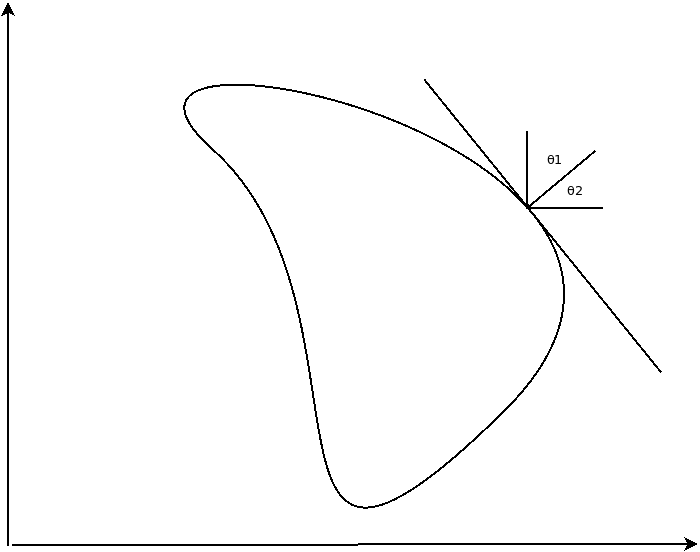
\includegraphics[scale=0.42]{./fig1.png} 
\end{center} 
\caption{Visualización ángulos $\theta_1$ y $\theta_2$}
\label{fig::fig1}
\end{figure}
Algunos problemas en física en áreas como mecánica de sólidos y elasticidad tienen ecuaciones diferenciales parciales asociadas similares a \ref{eq::partial_diff_equation}. La solución a este problemas de este tipo típicamente minimizan cierto funcional, que involucra integrales definidas, sobre una clase de funciones determinada por el problema.\\

Al suponer que $p,q,r$ y $f$ son todas continuas en $\mathcal{D}\cup\mathcal{S}$, $p$ y $q$ tiene primeras derivadas parciales continuas, y $g_1$ y $g_2$ son continuas en $\mathcal{S}_2$. Adicionalmente se supone que $p(x,y)>0, \, q(x,y)>0,\,r(x,y)\leq 0$ y $g_1(x,y)>0$. Entonces la solución de \ref{eq::partial_diff_equation} minimiza el funcional $I[w]$ únicamente, i.e. está es la única función que minimiza al funcional.
\begin{equation}\label{eq::functional}
\begin{aligned}
I[w]=\int\int_{\mathcal{D}}\Bigg\{ \frac{1}{2}\Big[p(x,y)\Big( \frac{\partial w}{\partial x} \Big)^2 + q(x,y)\Big( \frac{\partial w}{\partial y} \Big)^2 -r(x,y) w^2 \Big] +f(x,y)w\Bigg\}dx dy\\
+\int_{\mathcal{S}_2}\Bigg\{ -g_2(x,y)w+\frac{1}{2}g_1(x,y)w^2 \Bigg\}dS
\end{aligned}
\end{equation}
sobre todas las funciones dos veces diferenciables y continuas $w$ que satisfacen la ecuación \ref{eq::boundary1} en $\mathcal{S}_1$. El método de elementos finitos aproxima está solución al minimizar al funcional I \ref{eq::functional} sobre una clase mas pequeña de funciones, similar al acercamiento utilizado el método de Rayleigh-Ritz(ver Burden. \cite{Burden}).
\subsection{Definiendo los elementos finitos}
El primer paso es de definir los elementos finitos para construir la aproximación, esto consiste en dividir la región en un número finito de secciones o elementos con una forma regular, pueden ser triángulos, rectángulos, o cualquier figura regular que "tesele" o discretice la región por completo(\textit{tiling the region}).\\

El conjunto de funciones regularmente usadas para la aproximación es un conjunto de polinomios por partes de grado fijo en $x$ y $y$, y la aproximación requiere que los polinomios sean unidos de tal manera que la función resultante sea continua con primera y segunda derivadas integrables sobre la región entera. polinomios de tipo linear en $x$ y $y$ 
\begin{equation}
\phi(x,y)=a+bx+cy
\end{equation}
se utilizan comúnmente con elementos triangulares, mientras que polinomios de tipo bilinear en $x$ y $y$
\begin{equation}
\phi(x,y)=a+bx+cy+dxy
\end{equation}
están asociados al uso de elementos rectangulares.\\

Suponiendo que la región $\mathcal{D}$ ha sido subdividida en elemento triangulares. El conjunto de triángulos se denota como $D$, y los vértices de dichos triángulos se llaman nodos. El método busca una aproximación de la forma 
\begin{equation}
\phi(x,y)=\sum_{i=1}^{m}\gamma_i \phi_i(x,y),
\end{equation}
donde $\phi_1,\phi_2,\hdots,\phi_m$ son polinomios lineales por partes linealmente independientes, y las $\gamma_1, \gamma_2,\hdots,\gamma_m$ son constantes. Algunas de estas constantes, por ejemplo $\gamma_{n+1}, \gamma_{n+2},\hdots,\gamma_m$ se utilizan para asegurar que la condición de frontera 
\begin{equation}\label{eq::phi}
\phi(x,y)=g(x,y)
\end{equation}
se satisfaga en $\mathcal{S}_1$, las constantes restantes $\gamma_1,\gamma_2,\hdots,\gamma_n$, se utilizan para minimizar el funcional $I[\sum_{i=1}^m \gamma_i \phi_i]$. Usando la forma de \ref{eq::phi} para la aproximación de $w$ en la expresión \ref{eq::functional} se obtiene
\begin{equation}\label{eq::aproximated_functional}
\begin{aligned}
I[\phi]&=I\Big[ \sum_{i=1}^{m} \gamma_i \phi_i \Big]\\
&=\int\int_{\mathcal{D}}\Bigg(\frac{1}{2}\Bigg\{ p(x,y)\Big[ \sum_{i=1}^{m}\gamma_i \frac{\partial \phi_i}{\partial x}(x,y)\Big]^2 + q(x,y)\Big[ \sum_{i=1}^{m}\gamma_i \frac{\partial \phi_i}{\partial y}(x,y)\Big]^2\\
&-r(x,y)\Big[ \sum_{i=1}^{m}\gamma_i \phi_i(x,y)\Big]^2\Bigg\}+f(x,y)\sum_{i=1}^m \gamma_i \phi_i(x,y)\Bigg)dy\, dx\\
&^+\int_{\mathcal{S}_2}\Bigg\{ -g_2(x,y)\sum_{i=1}^m \gamma_i \phi_i(x,y)+\frac{1}{2}g_1(x,y)\Big[\sum_{i=1}^m \gamma_i \phi_i(x,y)\Big]^2\Bigg\}dS
\end{aligned}
\end{equation}
Como se menciono anteriormente se utiliza $\gamma_i, \gamma_2,\hdots, \gamma_n$ para minimizar el funcional, con esto al considerar a $I$ como una función de $\gamma_i, \gamma_2,\hdots, \gamma_n$, i.e. $I[\gamma_i, \gamma_2,\hdots, \gamma_n]$. Para que obtener un mínimo se tiene que cumplir
\begin{equation}\label{eq::minimun_condition}
\frac{d I}{d \gamma_j}=0,\,\, \forall\, j=1,2,\hdots,n.
\end{equation}

Diferenciando \ref{eq::aproximated_functional} con respecto $\gamma_i$ se obtiene
\begin{equation}
\begin{aligned}
\frac{\partial I}{\partial \gamma_i}=&\int \int_{\mathcal{D}}\Bigg\{p(x,y)\sum_{i=1}^m \gamma_i\frac{\partial \phi_i}{\partial x}(x,y)\frac{\partial \phi_j}{\partial x}(x,y)\\
& + q(x,y)\sum_{i=1}^{m}\gamma_i\frac{\partial \phi_i}{\partial y}(x,y)\frac{\partial \phi_j}{\partial y}(x,y)\\
& - r(x,y)\sum_{i=1}^{m}\gamma_i \phi_i(x,y)\phi_j(x,y)+f(x,y)\phi_j(x,y)\Bigg\}dx\,dy\\
& + \int_{\mathcal{S}_2}\Bigg\{-g_2(x,y)\phi_j(x,y)+g_1(x,y)\sum_{i=1}^m \gamma_i \phi_i(x,y)\phi_j(x,y)\Bigg\}dS,
\end{aligned}
\end{equation}
con esto la condición para minimizar el funcional se convierte en 
\begin{equation}
\begin{aligned}
0&=\sum_{i=1}^m \Bigg[\int \int_{\mathcal{D}}\Bigg\{ p(x,y) \gamma_i\frac{\partial \phi_i}{\partial x}(x,y)\frac{\partial \phi_j}{\partial x}(x,y)+ q(x,y) \gamma_i\frac{\partial \phi_i}{\partial y}(x,y)\frac{\partial \phi_j}{\partial y}(x,y)\\
&-r(x,y)\phi_i(x,y)\phi_j(x,y)\Bigg\}dx\,dy\\
&+ \int_{\mathcal{S}_2}g_1(x,y)\phi_i(x,y)\phi_j(x,y)dS\Bigg]\gamma_i\\
&+ \int\int_{\mathcal{D}} f(x,y)\phi_j(x,y)dx\,dy-\int_{\mathcal{S}_2} g_2(x,y)\phi_j(x,y)dS.
\end{aligned}
\end{equation}
para cada $i=1,2,\hdots,n$. Este conjunto de ecuaciones puede expresarse con una ecuación matricial
\begin{equation}
\mathbf{A}\vec{c}=\vec{b},
\end{equation}
donde $\vec{c}=(\gamma_1,\hdots,\gamma_n)^t$. Con $\mathbf{A}=(\alpha_{ij})$ y $\vec{b}=(\beta_1,\hdots,\beta_n)^t$ son definidos a continuación
\begin{equation}\label{eq::alpha_ij}
\begin{aligned}
\alpha_{ij}=\int\int_{\mathcal{D}}\Bigg[ p(x,y)\frac{\partial \phi_i}{\partial x}(x,y)\frac{\partial \phi_j}{\partial x}(x,y)+ q(x,y)\frac{\partial \phi_i}{\partial y}(x,y)\frac{\partial \phi_j}{\partial y}(x,y)\\
-r(x,y)\phi_i(x,y)\phi_j(x,y)\Bigg] dx\,dy+\int_{\mathcal{S}_2} g_1(x,y)\phi_i(x,y)\phi_j(x,y)dS,
\end{aligned}
\end{equation}
para cada $i=1,2,\hdots,n$ y $j=1,2,\hdots,m$, y
\begin{equation}\label{eq::beta_i}
\beta_i=-\int\int_{\mathcal{D}}f(x,y)\phi_i(x,y) dx\,dy+\int_{\mathcal{S}} g_2(x,y)\phi_i(x,y)dS-\sum_{k=n+1}^m\alpha_{ik}\gamma_k.
\end{equation}
para cada $i=1,\hdots,n$.\\

La elección del conjunto de funciones base es de bastante importancia ya que la elección apropiada puede frecuentemente hacer que la matriz $\mathbf{A}$ sea positiva definida y tenga la forma de una matriz banda(\textit{banded matrix}). Para el problema de segundo orden \ref{eq::partial_diff_equation}, se asume que $\mathcal{D}$ es poligonal, de tal manera que $\mathcal{D}=D$, y que $\mathcal{S}$ es un conjunto de lineas rectas contiguas.

\subsection{Triangulando la región}
Para empezar el procedimiento delineado anteriormente es crucial el paso de subdividir la región $D$ en un conjunto de triángulos  $T_1,T_2,\hdots,T_M$ donde el triángulo $i$(i-esimo) tiene tres vértices o nodos que se denotan 
\begin{equation}\label{eq::triangle_vertex}
V_j^{(i)}=\big( x_j^{(i)},y_j^{(i)} \big),\,\,\, \text{para }\, j=1,2,3.
\end{equation}
Para simplificar la notación se escribe $V^{(i)}_j=\big(x_j^{(i)},y_j^{(i)})$ cuando se trabaja con el triángulo fijo $T_i$. En cada vértice $V_j$ hay un polinomio lineal asociado
\begin{equation}
N_j^{(i)}(x,y)\equiv N_j(x,y)=a_j+b_jx+c_jy,\,\,\,\text{donde }\, N_j^{(i)}(x_k,y_k)=
\begin{cases}
1, \,\,j=k\\
0, \,\,j\neq k
\end{cases}
\end{equation}
Este esquema produce un sistema linear de la forma
\begin{equation}\label{eq::vertex_equation}
\begin{bmatrix}
1 & x_1 & y_1\\
1 & x_2 & y_2\\
1 & x_3 & y_3
\end{bmatrix}
\begin{bmatrix}
a_j\\
b_j\\
c_j
\end{bmatrix}=
\begin{bmatrix}
0\\
1\\
0
\end{bmatrix}.
\end{equation}
En \ref{eq::vertex_equation} $j=2$ por lo que el elemento 1 ocurre en la fila 2, en general el elemento 1 ocurre en la fila $j$.\\

Sí se tienen un etiquetado de los nodos $E_1,\hdots,E_n$ que están en $D\cap \mathcal{S}$. Con cada nodo $E_k$ se asocia una función $\phi_k$ que es lineal en cada triángulo , tiene valor 1 en $E_k$, y es $0$ en los otros nodos(por construcción). Esta elección particular hace a $\phi_k$ idéntica a $N_j^{i}$ en el triángulo $T_i$ cuando el nodo $E_k$ es el vértice denotado por $V_j^{(i)}$.

\section{Formulación débil para FEM}
Para empezar la discusión de la formulación débil se inicia planteando el problema original también conocido como formulación fuerte, en este caso se considera a la ecuación diferencial parcial elíptica es decir la ecuación de Poisson
\begin{equation}\label{eq::strong_form}
\nabla^2 T= f(x)
\end{equation}
Con condición de Dirichlet 
\begin{equation}
T=u(x), \,\,\,\,x\in \Gamma_D
\end{equation}
y condición de Von Neumman
\begin{equation}
\nabla T \cdot \mathbf{n}=g(x),\,\,\,x\in \Gamma_N
\end{equation}
donde $\Omega\in \mathbb{R}$ es el dominio de la solución con contorno $d\Omega$, $\Gamma_D$ es la parte del contorno donde se aplica la condición de Dirichlet y $\Gamma_N$ es la parte del contorno con condiciones de Neumann, $T(x)$ es la función desconocida a encontrar o aproximar, $f(x), u(x), g(x)$ son funciones conocidas.\\
La forma débil de la ecuación \ref{eq::strong_form} se construye al realizar la integral
\begin{equation}
\int_{\Omega}(\nabla^2 T -f)\cdot s\, d\Omega=0
\end{equation}
donde $s$ es una función de prueba, integrando por partes se obtiene
\begin{equation}
\begin{aligned}
0&=\int_{\Omega}(\nabla^2 T -f)\cdot s\, d\Omega=\int_{\Omega}\nabla\cdot\big( \nabla T \big)\cdot s\, d\Omega-\int_{\Omega}f\cdot s d\Omega=\\
&=-\int_{\Omega}\nabla T \cdot \nabla s \,d\Omega + \int_{\Omega}\nabla\cdot\big(\nabla T \cdot s  \big)\,d\Omega-\int_{\Omega} f\cdot s\, d\Omega
\end{aligned}
\end{equation}
aplicando la ley de Gauss se obtiene
\begin{equation}
\int_{\Omega}\nabla \cdot T \nabla s d\Omega = \int\limits_{\Gamma_D \cup \Gamma_N} s \cdot(\nabla\cdot \mathbf{n})\, d\Gamma-\int_{\Omega}f\cdot s\, d\Omega
\end{equation}
la integral de superficie se puede separar en una integral para la parte de la superficie donde aplica la condición de Dirichlet y otra para la parte donde aplica la condición de Neumann
\begin{equation}\label{eq::intial_weak_form}
\int_{\Omega}\nabla  T \cdot \nabla s\, d\Omega = \int\limits_{\Gamma_D} s \cdot(\nabla\cdot \mathbf{n})\, d\Gamma+\int\limits_{\Gamma_N} s \cdot(\nabla\cdot \mathbf{n})\, d\Gamma-\int_{\Omega}f\cdot s\, d\Omega
\end{equation}
La ecuación \ref{eq::intial_weak_form} es la forma débil inicial de la ecuación de Poisson, pero no se puede aplicar directamente sin considerar primero las condiciones de frontera.

\subsection{Condiciones de contorno de Dirichlet}
En la parte de la superficie donde se aplican las condiciones de Dirichlet se tienen dos restricciones. Una de ella es la condición de frontera $T(x)=u(x)$ y la segunda es la integral de superficie sobre $\Gamma_D$ en la ecuación \ref{eq::intial_weak_form}. Para evadir el término de la integral de superficie solo se usa la condición en la frontera,  para lograr esto se toma a la función $T \in V(\Omega)$ y la función de prueba $s\in V_0(\Omega)$, donde
\begin{equation*}
\begin{aligned}
V(\Omega)=\{ &v(x)\in H^1(\Omega)\},\\
V_0(\Omega)=\{v(x) \in& H^1(\Omega);\, v(x)=0,\, x\in\Gamma_D\}.
\end{aligned}
\end{equation*}
Es decir que la función desconocida $T$ debe ser continua conjuntamente con su gradiente en el dominio de interés. Por el otro lado la función de prueba $s$ también debe ser continua al igual que su gradiente pero es cero en la superficie $\Gamma_D$.\\
Con este requerimiento el término relacionado a la integral de superficie se desvanece y la forma débil de la ecuación de Poisson para $T\in V(\Omega)$ y $s\in V_0(\Omega)$ es
\begin{equation}
\begin{aligned}
\int_{\Omega}\nabla \cdot T \nabla s d\Omega = \int\limits_{\Gamma_N} s \cdot(\nabla\cdot \mathbf{n})\, d\Gamma-\int_{\Omega}f\cdot s\, d\Omega\\
T(x)=u(x),\,\,\, x\in \Gamma_D.
\end{aligned}
\end{equation}
Por esta razón en la terminología de FEM(o en la amplia literatura sobre el método de elementos finitos) se conoce a las condiciones de Dirichlet como \textit{Condiciones esenciales de contorno}, ya que no están incluidas naturalmente en la formulación débil y tienen que usarse que imponerse tal cual.
\subsection{Condiciones de contorno de Neumann}
Las condiciones de contorno de Neumann corresponden al flujo conocido $g(x)=\nabla T \cdot\mathbf{n}$. La integral sobre la superficie de Neumann en la ecuación \ref{eq::intial_weak_form} contiene exactamente el mismo flujo, por lo que en este caso se puede hacer uso directo de la función $g(x)$ en la integral
\begin{equation}
\int_{\Omega} \nabla T\cdot \nabla s \, d\Omega= \int_{\Gamma_N}g\cdot s \, d\Gamma-\int_{\Omega}f\cdot s\,d\Omega,
\end{equation}
donde la función de prueba $s$ también pertenece al espacio $V_0$.\\
Por esto en la terminología de FEM se conoce a las condiciones de Neumann como \textit{Condiciones naturales de contorno} ya forman parte de la formulación débil.
\subsection{Formulación débil para la ecuación de Poisson}
Con los resultados anteriores se puede hacer la formulación débil de la ecuación de Poisson \ref{eq::strong_form}. Para cualquier función de prueba $s\in V_0(\Omega)$ hallar $T \in V(\Omega)$ tal que 
\begin{equation}
\begin{aligned}\label{eq::Poisson_weak_formulation}
\int_{\Omega} \nabla T\cdot \nabla s \, d\Omega= \int_{\Gamma_N}g\cdot s \, d\Gamma-\int_{\Omega}f\cdot s\,d\Omega,\\
T(x)=u(x),\,\,\,x\in\Gamma_D.
\end{aligned}
\end{equation}
\section{Análisis de implementaciones}
En está sección se hace un análisis de las implementaciones del método de diferencias finitas utilizando \textbf{Wolfram Mathematica 12} y \textbf{Python}, específicamente se utiliza la librería \textbf{FEniCS}(ver \cite{FEniCS}). Para hacer las comparaciones se han elegido tres ecuaciones diferenciales parciales:
\begin{itemize}
\item Ecuación Elíptica
\item Ecuación Hiperbólica
\item Ecuación Parabólica

\end{itemize}
\subsection{Ecuación Elíptica}
La ecuación diferencial parcial elíptica a resolver es la siguiente
\begin{equation}\label{eq::elliptic_pde}
\begin{aligned}
\nabla^2 u(x,y)&=x e^y\\
\frac{\partial ^2 u}{\partial x^2}+\frac{\partial ^2 u}{\partial y^2}&=x e^y, \,\,\, 0<x<2,\,\,0<y<1
\end{aligned}
\end{equation}
con condiciones de contorno
\begin{equation}
\begin{aligned}
u(0,y)=0,\,\,\,u(2,y)=2e^y,\,\,\,0\leq y\leq 1,\\
u(x,0)=x,\,\,\,u(x,1)=ex,\,\,\,0\leq x\leq 2.
\end{aligned}
\end{equation}
La ecuación elíptica es la famosa ecuación de Poisson, en este caso se está considerando un problema bidimensional.\\
\subsubsection{Implementación en Mathematica}
Al resolver está ecuación \ref{eq::elliptic_pde} con el paquete \texttt{Needs["NDSolve`FEM`"]} de \texttt{Wolfram Mathematica 12} se obtiene la siguiente solución numérica que se puede visualizar como una superficie embedida en el espacio tridimensional.
\begin{figure}[H]
\begin{center}
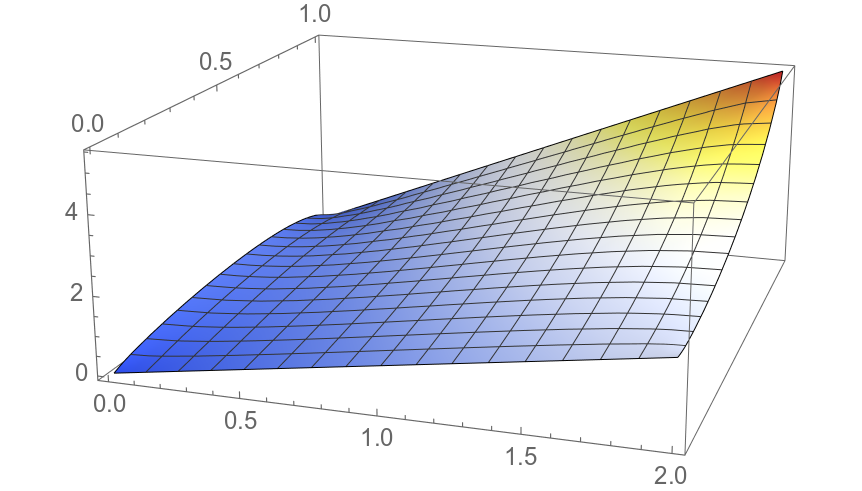
\includegraphics[scale=0.42]{./elliptic.png} 
\end{center} 
\caption{Visualización solución numérica de la EDP Elíptica}
\label{fig::fig2}
\end{figure}
Para hacer uso de las funcionalidades del paquete de método de elementos finitos incluido en \texttt{Mathematica} se puede definir una región para resolver a la ecuación elíptica mucho más interesante, digamos que queremos resolver la ecuación en la región rectangular definida anteriormente pero se quieren excluir los puntos que están dentro del circulo definidos por la desigualdad
\begin{equation}\label{eq::region1}
(x-0.2)^2+(y-0.2)^2\leq 0.3^2
\end{equation}
se obtiene la siguiente región en el plano
\begin{figure}[H]
\begin{center}
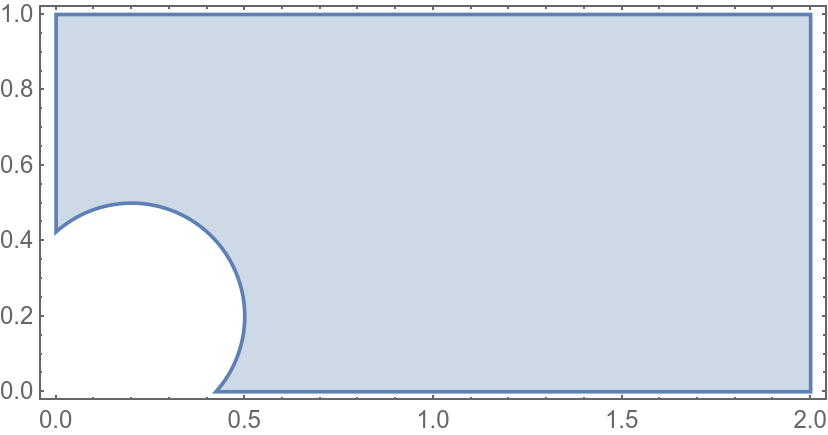
\includegraphics[scale=0.42]{./elliptic_omega.png} 
\end{center} 
\caption{Región que excluye los punto en la expresión \ref{eq::region1}}
\label{fig::fig3}
\end{figure}
Además de hacer la región más compleja se quieren imponer condiciones de Dirichlet de la forma
\begin{equation}
u(x,y)=
\begin{cases}
0, \,\,\, x=2,\,\,\,\,0.8\leq y \leq 1.0\\
10, \,\,\, (x-0.2)^2+(y-0.2)^2\leq 0.3^2
\end{cases}
\end{equation}
al resolver se obtiene las siguientes curvas de nivel
\begin{figure}[H]
\begin{center}
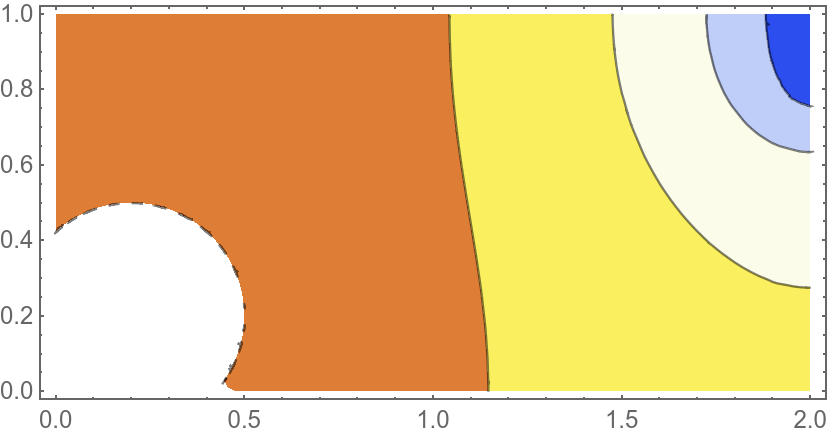
\includegraphics[scale=0.42]{./elliptic_omega_contour.png} 
\end{center} 
\caption{Curvas de nivel}
\label{fig::fig3}
\end{figure}
y la solucion correspondiente en el espacio tridimensional se puede visualizar a continuación
\begin{figure}[h]
\begin{center}
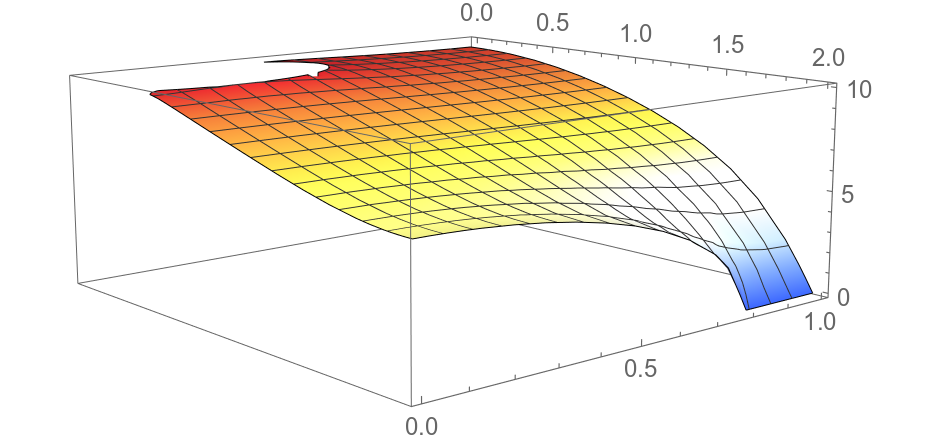
\includegraphics[scale=0.42]{./elliptic_omega_3D.png} 
\end{center} 
\caption{Solución numérica con condiciones de Dirichlet}
\label{fig::fig3}
\end{figure}
Se puede observar en este caso particular la teselación de la región de interés generada por el paquete anteriormente mencionado
\begin{figure}[H]
\begin{center}
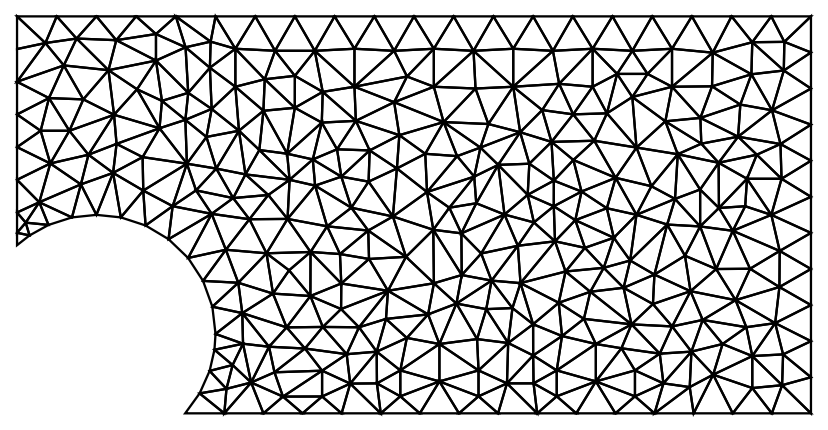
\includegraphics[scale=0.42]{./elliptic_omega_mesh.png} 
\end{center} 
\caption{Teselación de la región de interés}
\label{fig::fig4}
\end{figure}
\subsubsection{Implementación en FEniCS}
Para hacer uso del paquete \texttt{FEniCS} es necesario usar la formulación débil para EDP, como se expuso previamente para la ecuación elíptica o de Poisson se puede usar los términos en la integral \ref{eq::Poisson_weak_formulation} para escribir el código correspondiente.\\
Usando el problema \ref{eq::elliptic_pde} se obtiene el siguiente resultado para la aproximación de la solución que se puede visualizar en la siguiente figura
\begin{figure}[H]
\begin{center}
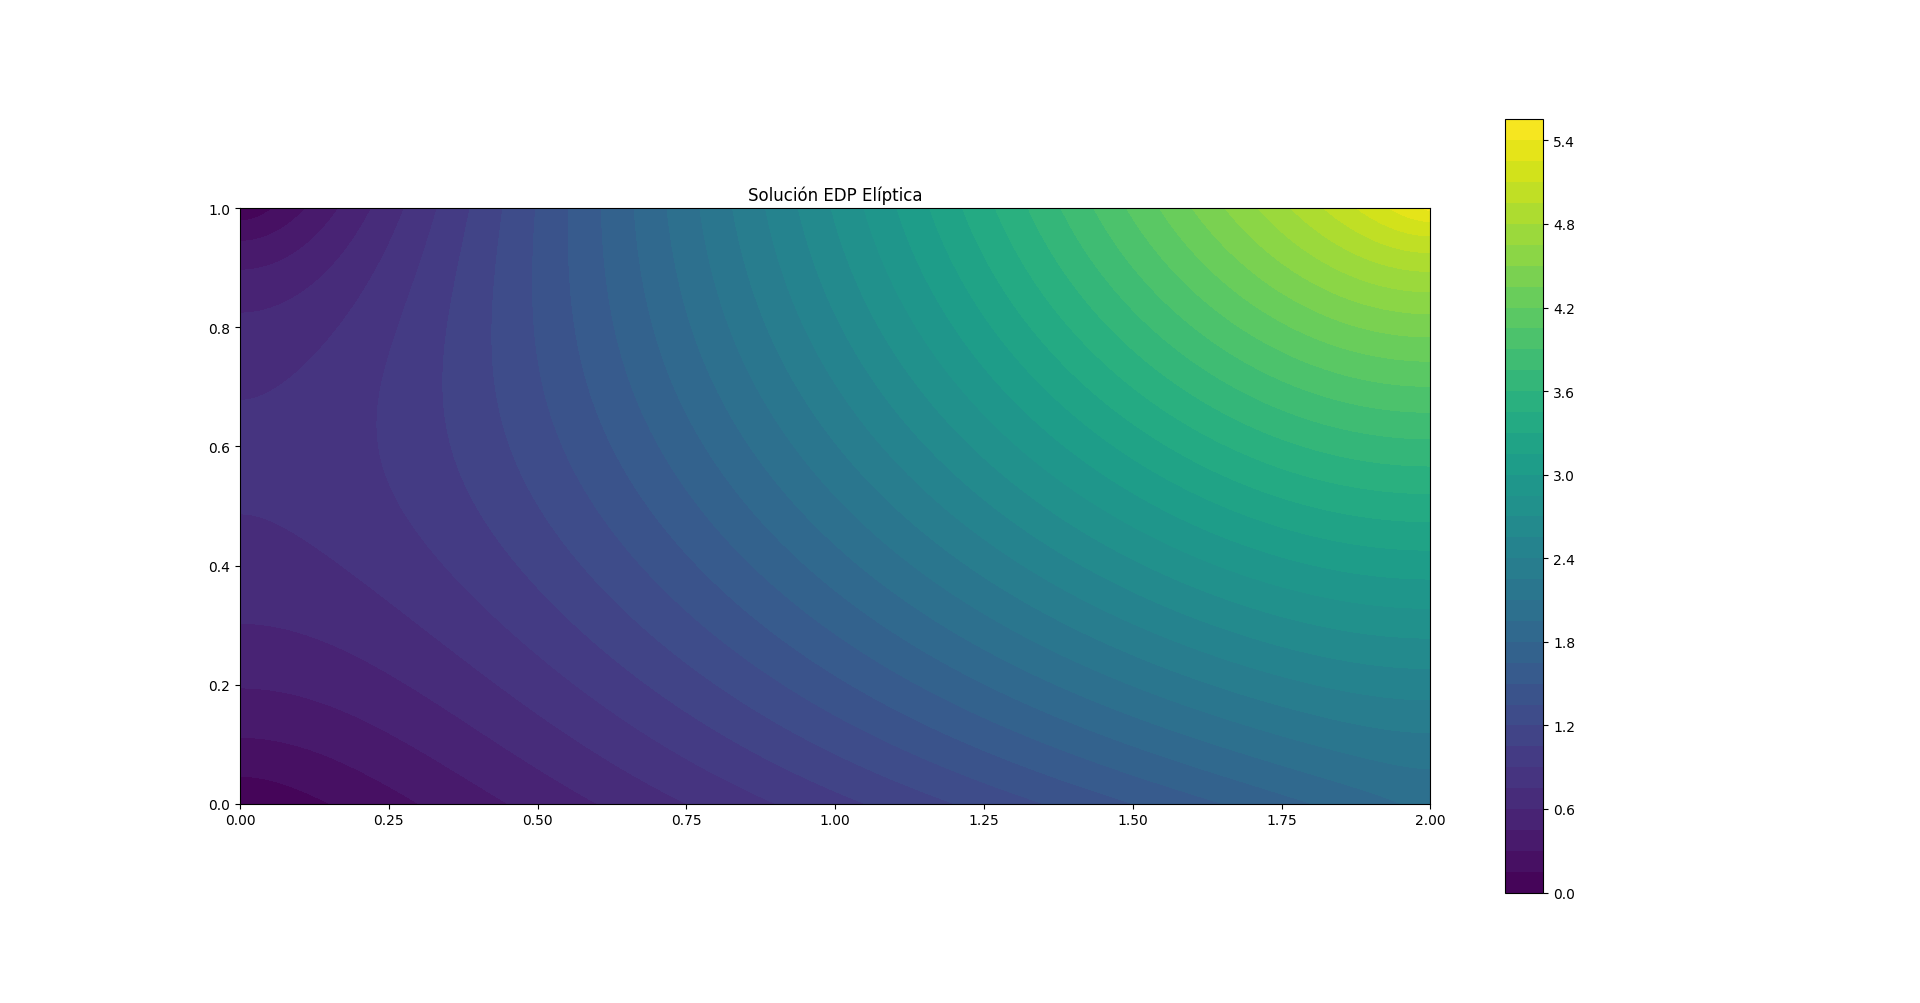
\includegraphics[scale=0.3]{./elliptic_FEniCS.png} 
\end{center} 
\caption{Solución numérica de la ecuación de Poisson}
\label{fig::fig4.2}
\end{figure}


\subsection{Ecuación Parabólica}
Para la ecuación parabólica se tiene el siguiente problema
\begin{equation}\label{eq::parabolic_pde}
\frac{\partial u}{\partial t}(x,t)-\frac{\partial^2 u}{\partial x^2}(x,t)=0,\,\,\,\,0<x<1,\,\,\,t\geq 0
\end{equation}
con condiciones de frontera
\begin{equation}
u(0,t)=u(1,t)=0,\,\,\,t>0
\end{equation}
y condiciones iniciales
\begin{equation}
u(x,0)=\sin(\pi x),\,\,\, 0 \leq x \leq 1
\end{equation}
\subsubsection{Implementación en Mathematica}
De nuevo utilizando el paquete \texttt{Needs["NDSolve`FEM`"]} y la función \texttt{NDSolveValue} se puede especificar de una manera sencilla el problema con sus condiciones de frontera e iniciales, el resultado se puede visualizar de mejor manera como una gráfica de la aproximación numérica 
\begin{figure}[H]
\begin{center}
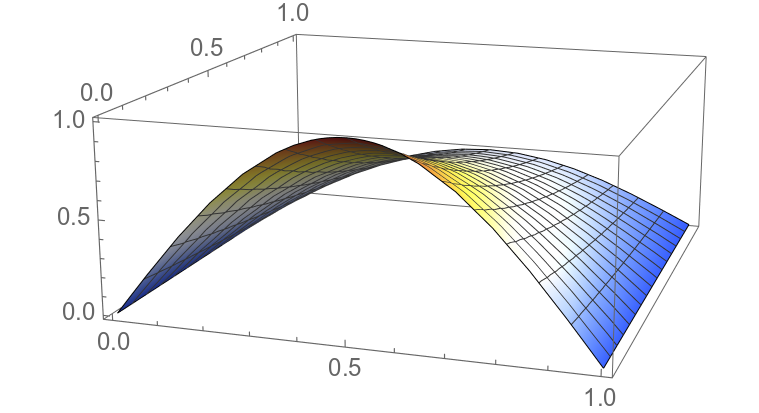
\includegraphics[scale=0.42]{./parabolic.png} 
\end{center} 
\caption{Aproximación numérica de la EDP parabólica}
\label{fig::fig5}
\end{figure}
Adicionalmente es útil visualizar las curvas de nivel de la solución numérica aproximada
\begin{figure}[H]
\begin{center}
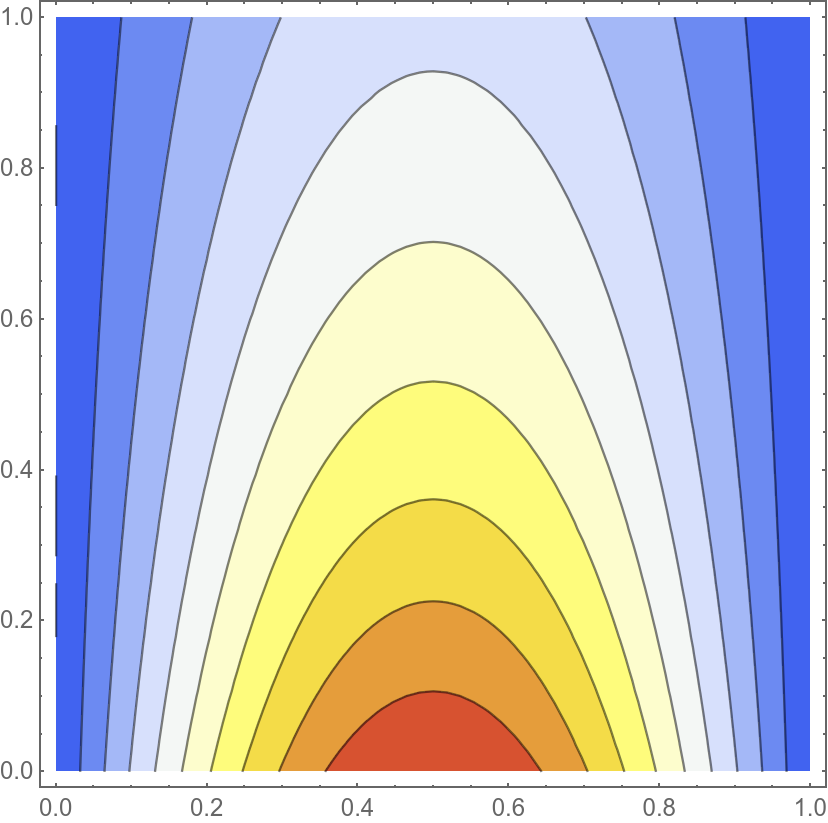
\includegraphics[scale=0.29]{./parabolic_contour.png} 
\end{center} 
\caption{Curvas de nivel de la aproximación numérica de la EDP parabólica}
\label{fig::fig6}
\end{figure}
\subsubsection{Implementación en FEniCS}
De nuevo para poder programar la resolución numérica de la ecuación es necesario formular la versión débil del problema \ref{eq::parabolic_pde}, esto se puede revisar en el código de \texttt{Python} del repositorio de \texttt{GitHub}, ver \cite{Medina}.\\
El resultado obtenido con FEniCS se presenta en la siguiente figura
\begin{figure}[H]
\begin{center}
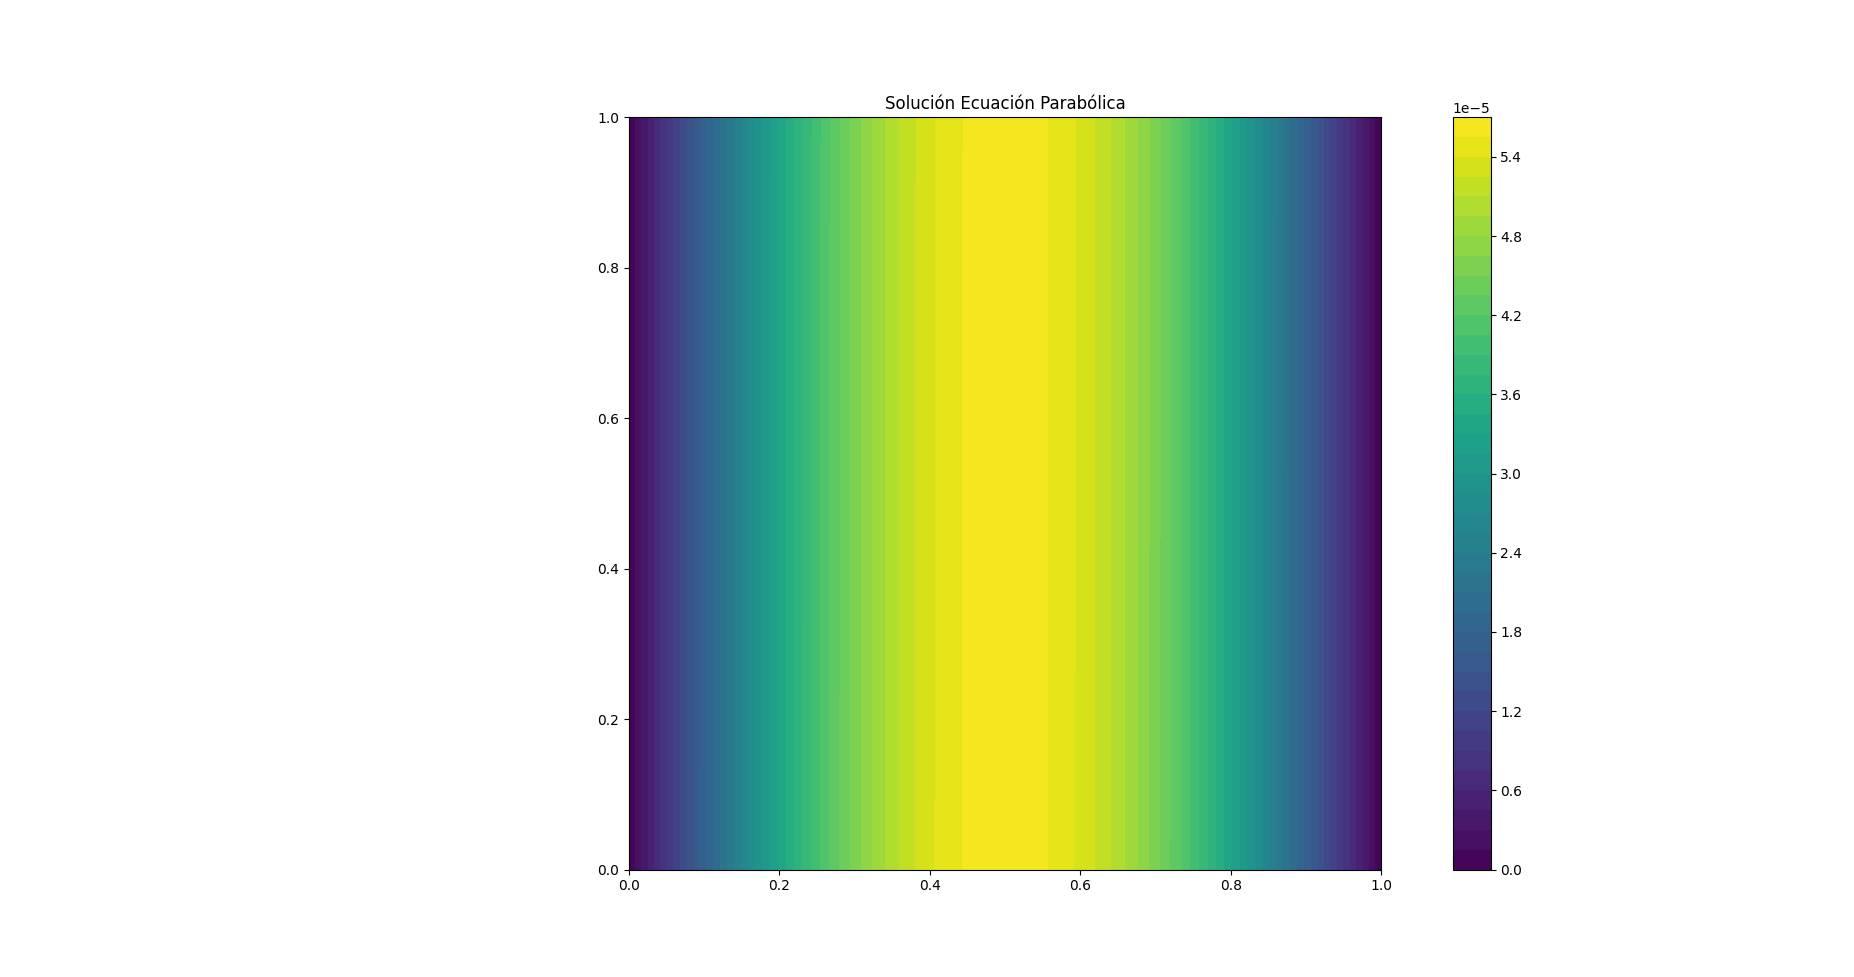
\includegraphics[scale=0.29]{./parabolic_FEniCS.png} 
\end{center} 
\caption{Aproximación para la solución de la EDP parabólica}
\label{fig::fig6}
\end{figure}
Para poder apreciar el tipo de teselación del espacio del dominio de interés creado con \texttt{FEniCS} se usa el retículo resultante sobre la solución anterior
\begin{figure}[H]
\begin{center}
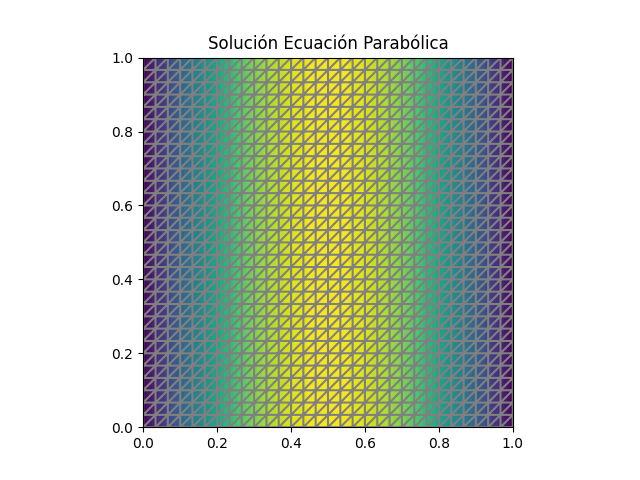
\includegraphics[scale=0.49]{./parabolic_FEniCS_mesh.png} 
\end{center} 
\caption{Teselación para la solución de la EDP parabólica}
\label{fig::fig7}
\end{figure}




\subsection{Ecuación Hiperbólica}
La ecuación hiperbólica también conocida como ecuación de onda. El problema a resolver para la ecuación diferencial parcial hiperbólica es 
\begin{equation} \label{eq::wave_equation}
\frac{\partial^2 u}{\partial t^2}(x,y)-4\frac{\partial ^2 u}{\partial x^2}(x,t)=0,\,\,\,0<x<1,\,\,\,t>0
\end{equation}
con condiciones de frontera 
\begin{equation}
u(0,t)=u(1,t)=0,\,\,\, \text{para, }\,\,t>0
\end{equation}
y condiciones iniciales
\begin{equation}
u(x,0)=\sin(\pi x), \,\,\, \text{y}\,\,\,\frac{\partial u}{\partial t}(x,0)=0,\,\,\, 0\leq x \leq 1
\end{equation}
\subsubsection{Implementación en Mathematica}
El resultado de resolver el problema \ref{eq::wave_equation} con las condiciones de frontera e iniciales en Mathematica se puede visualizar en la siguiente figura.
\begin{figure}[H]
\begin{center}
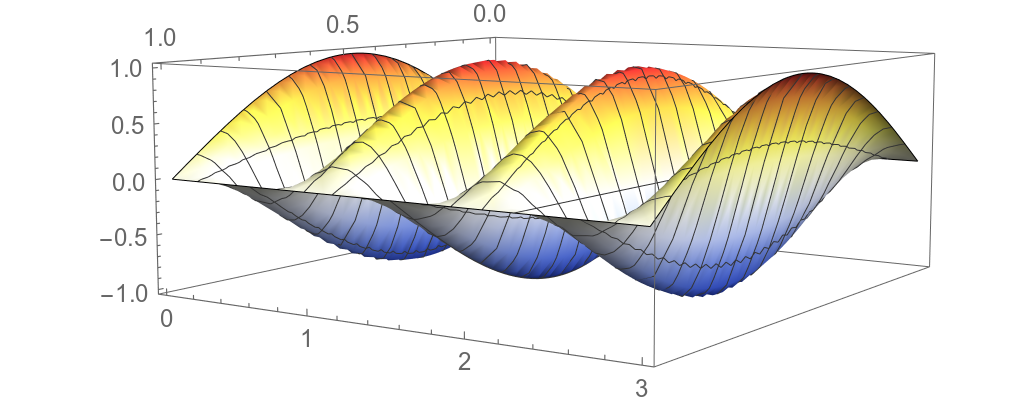
\includegraphics[scale=0.42]{./wave.png} 
\end{center} 
\caption{Solución numérica de la ecuación de onda}
\label{fig::fig7}
\end{figure}
Las curvas de nivel correspondientes se ven en la siguiente figura
\begin{figure}[H]
\begin{center}
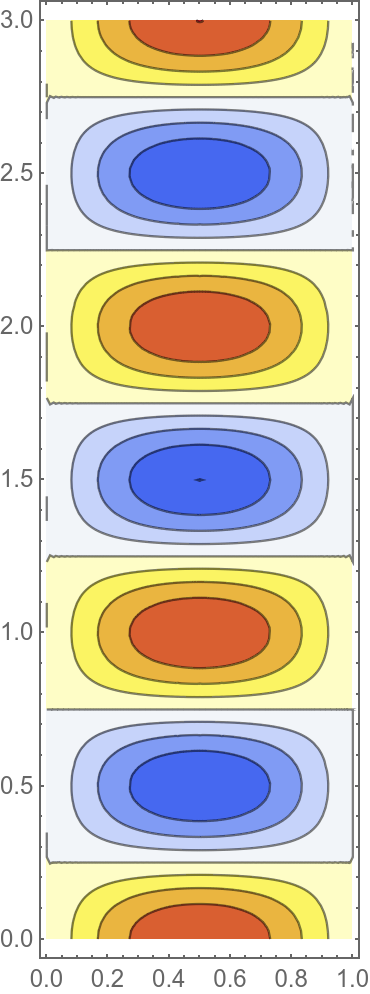
\includegraphics[scale=0.22]{./wave_contour.png} 
\end{center} 
\caption{Curvas de nivel para la solución numérica de la ecuación de onda}
\label{fig::fig8}
\end{figure}
\subsection{Implementación en FEniCS}
Utilizando la formulación débil de \ref{eq::wave_equation} se puede resolver el problema usando \texttt{FEniCS}, el resultado se presenta a continuación
\begin{figure}[H]
\begin{center}
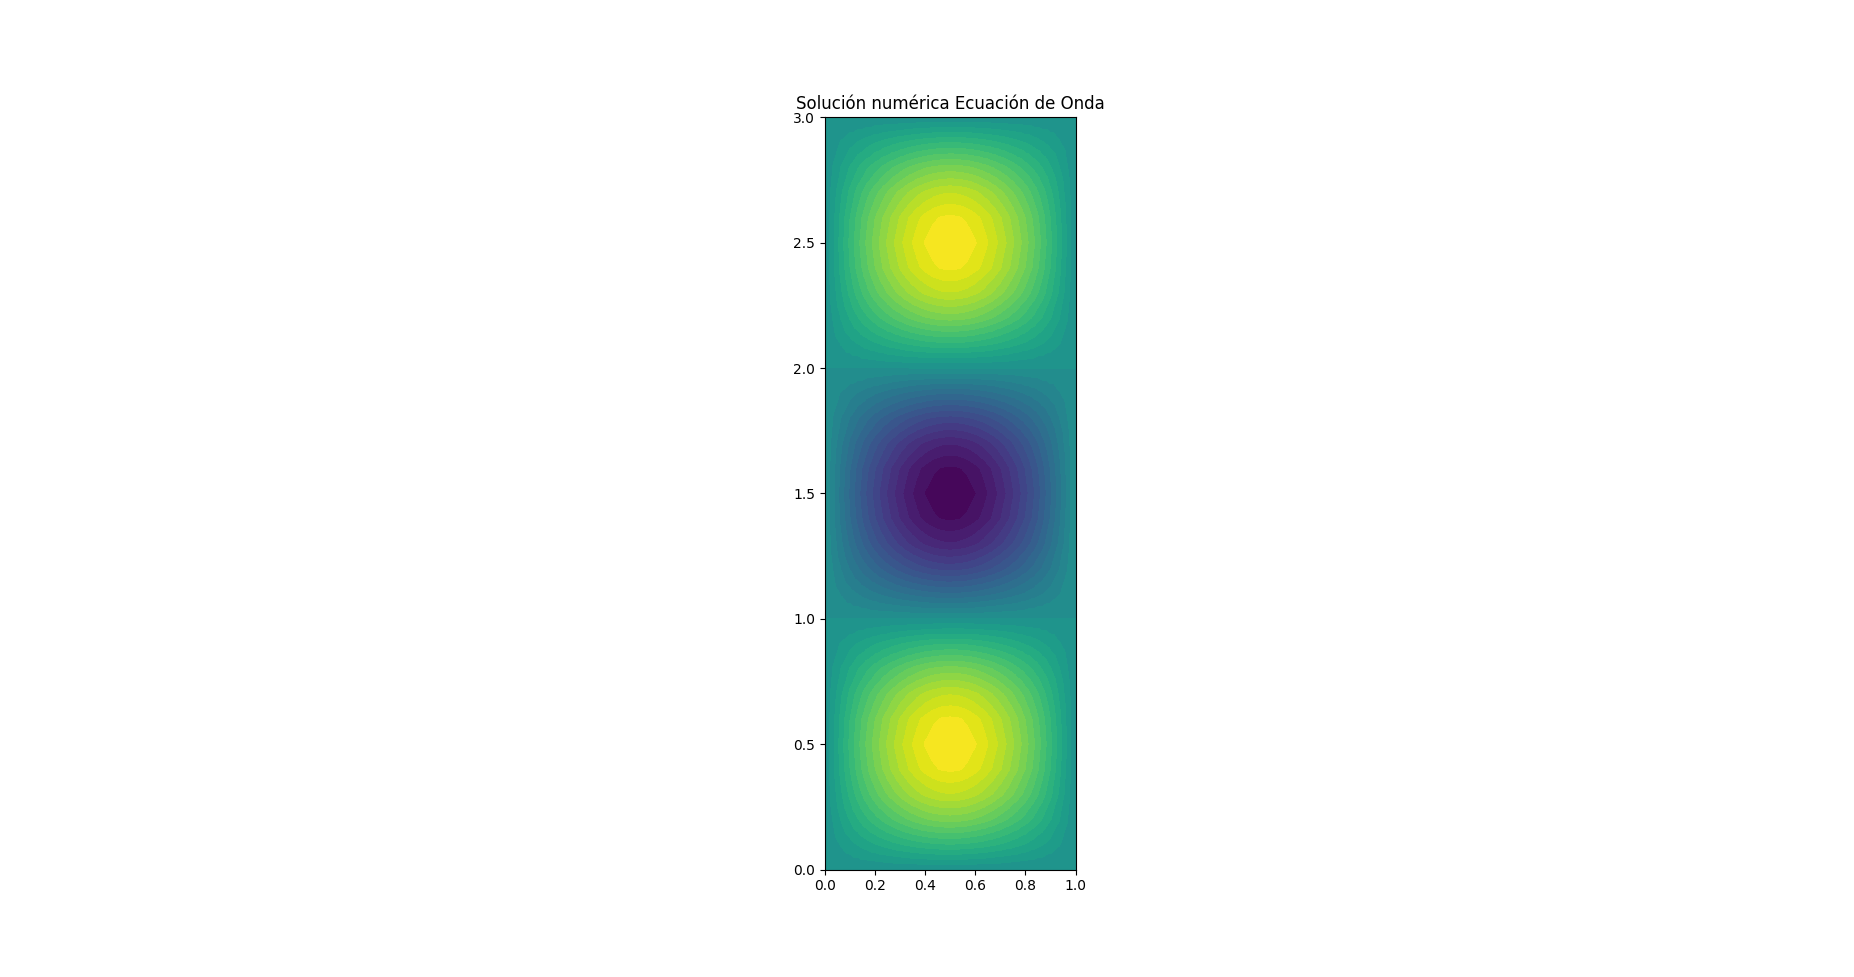
\includegraphics[scale=0.32]{./wave_FEniCS.png} 
\end{center} 
\caption{Curvas de nivel para la solución numérica de la ecuación de onda}
\label{fig::fig8}
\end{figure}
\section{Comparación de implementaciones}
Para poder comparar las implementaciones realizadas para las soluciones de las ecuaciones diferenciales parciales cónicas presentadas anteriormente se compara la memoria RAM utilizada en promedio por cada paquete.\\
\begin{center}
\begin{tabular}{ |c|c|c|c| } 
\hline
Ecuación Diferencial Parcial & \texttt{Wolfram Mathematica}& \texttt{Python/FEniCS}\\
\hline
Elíptica& $188$MB & $266$MB \\ 
Parabólica& $178$MB& $148$MB\\ 
Hiperbólica& $178$MB & $152$MB\\ 
\hline
\end{tabular}
\end{center}
\subsection{Discretización del espacio}
El paso de discretizar el dominio de interés es fundamental en el método de elementos finitos, hay muchos acercamientos teóricos de como lograr este objetivo. Como se discutió anteriormente la elección de la figura geométrica elemental para realizar la teselación tiene repercusiones directas en la construcción del método.\\

Para mencionar algunos de los métodos utilizado por el paquete \texttt{NeedsFEM} de \texttt{Wolfram Mathematica} se tienen los siguientes:
\begin{enumerate}
  \item \textbf{Triangulación de Delaunay}: Este es un algoritmo común utilizado en la generación de mallas 2D. Una triangulación de un conjunto de puntos es de Delaunay si ningún punto está dentro del círculo circunscrito de cualquier triángulo. Las triangulaciones de Delaunay maximizan el ángulo mínimo de todos los ángulos de los triángulos, lo que resulta en triángulos 'bien formados'.
  \item \textbf{Diagrama de Voronoi}: Este es un grafo dual a la triangulación de Delaunay. Dado un conjunto de puntos, para cada punto habrá un polígono donde todas las ubicaciones dentro del polígono están más cerca del punto dado que de cualquier otro. Los polígonos juntos forman un diagrama de Voronoi. Esto se puede usar en estrategias de refinamiento de mallas.
  \item \textbf{Método Octree (Quadtree en 2D)}: Este es un método común en la generación de mallas 3D. La idea es dividir recursivamente el dominio en ocho (cuatro en 2D) partes iguales hasta que se alcance la granularidad deseada. La transición entre diferentes niveles de granularidad puede ser manejada por elementos de transición especiales.
  \item \textbf{Método de Frente Avanzado}: Este método implica comenzar desde una malla de frontera y agregar gradualmente elementos al interior. Se mantiene un "frente" entre las áreas ya malladas y las áreas aún por mallas, y se agregan nuevos nodos de manera que este frente avance.
  \item \textbf{Algoritmo de Ruppert}: Esto es un refinamiento de la triangulación de Delaunay que además tiene en cuenta un criterio sobre el ángulo mínimo, lo que lleva a triangulaciones de alta calidad.
  

\end{enumerate}

\texttt{FEniCS} también utiliza algunas de las técnicas y marcos teóricos que utilizan en \texttt{Wolfram Mathematica} sin embargo siendo un proyecto \textit{open-source}(código abierto) hay alguna fortalezas que se pueden mencionar de su uso:
\begin{enumerate}
  \item \textbf{Generación de mallas}: Para el paso de generación de mallas, \texttt{FEniCS} utiliza bibliotecas como \texttt{mshr} y \texttt{CGAL} para crear y manipular mallas complejas.
  \item \textbf{Montaje de Elementos Finitos}: La principal fortaleza de \texttt{FEniCS} reside en su montaje automatizado de elementos finitos. \texttt{FEniCS} utiliza el concepto de formas variacionales (la base matemática de la discretización de elementos finitos) que se puede definir en notación casi matemática directamente en un programa de Python o C++.
  \item \textbf{Resolución de problemas}: \texttt{FEniCS} utiliza la biblioteca \texttt{PETSc} para la solución de sistemas de ecuaciones lineales y no lineales, una herramienta poderosa y escalable para estos cálculos.
\end{enumerate}

\section{Análisis estadístico en los resultados de una aproximación numérica}

El análisis estadístico se puede realizar en los resultados de una aproximación numérica para comprender mejor las características y el rendimiento del método de aproximación, validar los resultados e inferir sobre el proceso que generó los datos. Algunas técnicas estadísticas utilizadas comúnmente :

\begin{enumerate}
  \item \textbf{Estadísticas descriptivas}: Esto puede incluir la media, mediana, moda, desviación estándar, varianza, rango, mínimo, máximo, cuartiles y otras medidas que describen las características básicas de los datos. Esto puede dar una idea de la tendencia central, la dispersión y la distribución de los datos.
  \item \textbf{Análisis de error}: Puede calcular los residuos (la diferencia entre los valores observados y predichos) y analizar su distribución. Podría calcular el error absoluto medio, el error cuadrado medio u otras métricas de error. Podría ser útil trazar residuos para inspeccionar visualmente los patrones.
  \item \textbf{Intervalos de confianza}: Podría construir intervalos de confianza alrededor de sus parámetros estimados o predicciones para cuantificar la incertidumbre.
  \item \textbf{Pruebas de hipótesis}: Si tiene una hipótesis específica sobre sus resultados, como si un método de aproximación es superior a otro, podría realizar una prueba de hipótesis. Por ejemplo, se podría utilizar una prueba t para comparar las medias de dos grupos.
  \item \textbf{Análisis de correlación}: Si tiene varias variables en sus resultados, podría examinar las relaciones entre ellas utilizando coeficientes de correlación o diagramas de dispersión.
  \item \textbf{Análisis de regresión}: Si sus resultados se basan en múltiples variables de entrada, puede usar el análisis de regresión para entender cómo estas variables influyen colectivamente en el resultado. Esto también puede ayudarle a predecir resultados futuros.
  \item \textbf{Análisis de varianza (ANOVA)}: Si está comparando los resultados de diferentes métodos de aproximación o diferentes ajustes del mismo método, ANOVA se puede utilizar para determinar si las diferencias entre los grupos son estadísticamente significativas.
  \item \textbf{Bootstrap o validación cruzada}: Estas técnicas se pueden usar para estimar la precisión de su método de aproximación al remuestrear los datos o dividirlos en subconjuntos.
  \item \textbf{Análisis de Monte Carlo}: Si su aproximación numérica involucra aleatoriedad (como en la integración de Monte Carlo), entonces puede analizar la distribución de los resultados de múltiples ejecuciones para entender la media, la varianza y otras propiedades estadísticas.
\end{enumerate}

\section{Conclusiones}

El método de elementos finitos se ha convertido en una herramienta fundamental en el modelado matemático, en las simulaciones físicas y en análisis de ingeniería. Es bien conocida la dificultad para abordar problemas de ecuaciones diferenciales parciales con condiciones en la frontera(Dirichlet o Neumann) y encontrar soluciones analíticas a estos, una ejemplo iconico en la física a nivel de postgrado se puede dar con el estudio de problemas de la teoría electromagnética encontrados en Jackson \cite{Jackson}.\\

El uso de paquetes computacionales para abordar estos problemas es ubicuo en toda la ciencia, ya que la mayoría de problemas no se pueden resolver de manera analítica por lo que es obligatorio utilizar algún acercamiento numérico. Las ventajas expuestas en el manejo de las condiciones de frontera hacen que el método de elementos finitos sea una de las opciones más utilizadas en la práctica.\\

De los resultados obtenidos al resolver las ecuaciones cónicas se pueden establecer que \texttt{Wolfram Mathematica} y \texttt{FEniCS} tienen una implementación de FEM muy robusta y relativamente fácil de utilizar, cada uno tiene sus ventajas y desventajas. \texttt{Wolfram Mathematica} hace que la formulación del problema se pueda hacer casi de manera natural es decir que la sintaxis para definir al problema es muy similar a lo que se escribiría en una hoja de papel o en LaTeX, se escribe la EDP directamente. Para contrastar esto en \texttt{FEniCS} hay que elaborar un poco más y definir la formulación débil del problema. Uno es un software propietario y el otro de código abierto esto hace de \texttt{FEniCS} una opción más accesible y configurable a costo de un conocimiento más detallado de la programación. Las diferencias en el consumo de RAM especificamente para estos problemas no es significativa, sin embargo vale mencionar que tanto \texttt{Python} como \texttt{Mathematica} son bien conocidos por tener un consumo elevado de memoria RAM.\\
En cuanto a la rapidez de la soluciones el gran ganador es \texttt{Mathematica} ya resuelve los problemas casi instantáneamente mientras que en \texttt{Python} la solución puede tardar hasta un par de minutos dependiendo los parámetros utilizados. En este caso sería interesante usar \texttt{C++} para hacer una comparación de tiempos más razonable.



\begin{thebibliography}{99}
%% La bibliografía se ordena en orden alfabético respecto al apellido del 
%% autor o autor principal
%% cada entrada tiene su formatado dependiendo si es libro, artículo,
%% tesis, contenido en la web, etc


\bibitem{Burden} Richard L. Burden, J. Douglas Faires \textit{Numerical Analysis}, (Ninth Edition). Brooks/Cole, Cengage Learning. 978-0-538-73351-9

\bibitem{sfepy} Cimrman, R., Lukeš, V., Rohan, E., 2019. \textit{Multiscale finite element calculations in Python using SfePy}. Advances in Computational Mathematics 45, 1897-1921. https://doi.org/10.1007/s10444-019-09666-0

\bibitem{FEniCS}M. S. Alnaes, J. Blechta, J. Hake, A. Johansson, B. Kehlet, A. Logg, C. Richardson, J. Ring, M. E. Rognes and G. N. Wells.\textit{The FEniCS Project Version 1.5, Archive of Numerical Software 3 (2015)}. [doi.org/10.11588/ans.2015.100.20553]
\bibitem{}A. Logg, K.-A. Mardal, G. N. Wells. \textit{Automated Solution of Differential Equations by the Finite Element Method}, Springer(2012). [doi.org/10.1007/978-3-642-23099-8]

\bibitem{Medina}Julio Medina. \textit{Método de Elementos Finitos}. \url{https://github.com/Julio-Medina/Finite_Element_Method}

\bibitem{Jackson}  John David Jackson. \textit{Classical Electrodynamics}. Wiley, 1999.
%\bibitem{Feynman} 
%\bibitem{Hopfield} J.J. Hopfield. \textit{Neural Networks and physical systems with emergent collective computational abilities}. \url{https://doi.org/10.1073/pnas.79.8.2554}


%\bibitem{McCulloch} Warren S. McChulloch, Walter H. Pitts. \textit{A LOGICAL CALCULUS OF THE IDEAS IMMANENT IN NERVOUS ACTIVITY}. \url{http://www.cse.chalmers.se/~coquand/AUTOMATA/mcp.pdf}



\end{thebibliography}
\end{document}

